\subsection{Overview}
An essential part of the platform design is to satisfy not only functional requirements but non-functional requirements as well.This means that architectural choices are crucial at this point of the development for the sake of achieving the desired output in terms of requirements ,performance ,scalability and user experience.//
An important focus will be set on how the different systems interact with each other and the back-end to obtain the events as required by sec. 3 of the RASD.Furthermore choices regarding upscaling and redundancy will be discussed.//

\subsection{Component View}
This section focuses on the component overview giving an insight on their core functionality and various interfaces.//
\subsubsection{RESTful API}
The RESTful API is a gateway communicator between clients and the back-end system: it's a stateless service which provides methods for data submission or requests returning the requested computations as a result.//
RESTful API are an optimal solution for an application that must handle a vast number of users on a different number of platforms as it allows to guarantee the same user experience on all platforms. Furthermore the architectural properties positively affected by the constraints of the REST architectural include many important quality requirements such as performance, scalability and reliability.

\subsubsection{User manager}
This component handles user data, registration and authentication.The user manager has direct access to the DBMS and receives read and write requests from the RESTful API.
\subsubsection{Notification manager}
This component is responsible for implementing the push notification service towards
the user-side applications.
It is necessary to have this type of module running in the back-end because
there are cases in which a communication must happen between the clients and
the back-end, but no direct request is made to the RESTful API by the clients:
for example when the reserved car is nearby, the system must send the user a 'ready to unlock' notification.
\subsubsection{Vehicle manager}
The car manager component's job is to manage all the vehicles throughout the city.It can access the DBMS to query vehicle information but stores essential vehicle information locally such as location ,battery level and number of seats. When the search manager gets triggered it forwards requests to the vehicle manager to get all 
available car in compliance to the user input.
\subsubsection{Search manager}
The search manager component handles all incoming search requests forwarded by the user applications and interfaced through the RESTful API. The main functionality is to handle the user input and query the vehicle manager accordingly, returning the desired output to the user.\\In the event of a booking request the search manager forwards the demand to the Ride Manager.
\subsubsection{Ride Manager}
The Ride manager component examines all incoming reservation request and creates \textit{Ride objects} according to the user selection and user data.The ride manager
is connected to the following components:
\begin{itemize}
\item \textit{Vehicle manager}: need to communicate and receive communications about car status changes in terms of availability, battery level and location.
\item \textit{Notification manager}: need to inform the user about remaining time to unlock the car or send the user 'ready to unlock ' notifications. Moreover it sends messages to the on-board display to inform the user about the response to a \textit{end ride request}.
\item \textit{DBMS}: need to update the user reservation and payment history once a ride has been marked as completed.  
\end{itemize}
\subsubsection{Component diagram}
\begin{center}
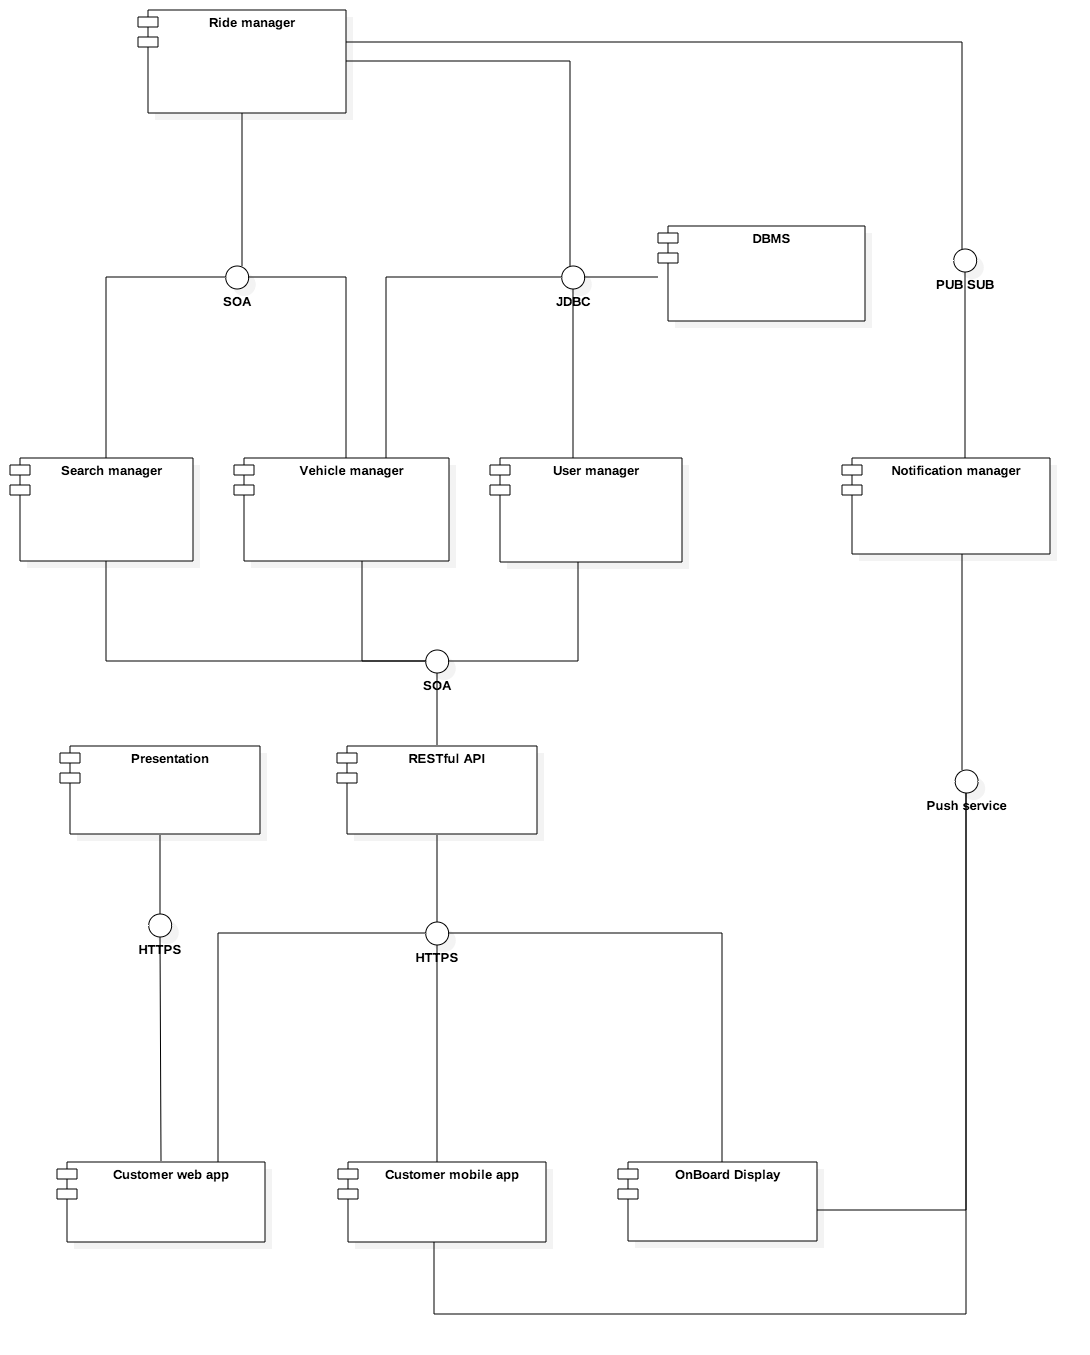
\includegraphics[scale=0.4]{Images/ComponentDiagram/ComponentDiagram.png}
\end{center}
\subsection{Deployment View}
\newpage
\subsection{Runtime View}
\newpage
\subsection{Component Interfaces}
\newpage
\subsection{Selected architectural styles and patterns}
\newpage
\subsection{Other design decisions}
\newpage